\documentclass[11pt]{article}
\usepackage[preprint]{acl}

\usepackage{times}
\usepackage{latexsym}
\usepackage[T1]{fontenc}
\usepackage[utf8]{inputenc}
\usepackage{microtype}
\usepackage{inconsolata}
\usepackage{graphicx}
\usepackage{booktabs}
\usepackage{algorithm}
\usepackage{algpseudocode}

\title{Tracing the Birth of a Fact: Exposure-Level Dynamics of Knowledge \\ Acquisition and Hallucination in LMEnt}

\author{
  Marah Assad \\
  Tel Aviv University \\
  \texttt{marahassad@mail.tau.ac.il}
}

\begin{document}
\maketitle

\begin{abstract}
Prior work shows that language models acquire factual knowledge in phases during pretraining and that hallucinations emerge alongside that knowledge, but these findings have relied on aggregate statistics (dataset frequency, duplication rate) rather than exact, per-fact exposure records. We use LMEnt \citep{gottesman2025lment}, a suite of small language models trained with full sequence-level provenance over an entity-annotated Wikipedia corpus, to track individual facts across training. For a set of PopQA-style facts \citep{mallen2023whennot}, we recover the exact training step at which each fact's supporting text was seen and compare this against the model's answer confidence at each of 12 checkpoints, evaluated with a multiple-choice-style probe against same-relation decoys. We find that (1) exposure frequency predicts how quickly a fact is learned, and this relationship gets \emph{stronger}, not weaker, when we repeat the experiment on a larger model (Pearson $r$ rises from 0.34 at 170M parameters to 0.50 at 600M); (2) both models show a rise-then-partial-decline accuracy trajectory consistent with the ``forgetting'' dynamic reported by \citet{chang2024howdo}, and we confirm via a decoy-substitution check that this is not an artifact of our evaluation; and (3) the decline is markedly less pronounced in the larger model, suggesting it is at least partly a small-model capacity effect rather than a fundamental property of the training dynamics. A separate test of whether \emph{recency} of last exposure, rather than raw count, predicts forgetting was inconclusive -- a negative result we report rather than omit.
\end{abstract}

\section{Introduction}

Large language models store an enormous amount of factual knowledge in their parameters, yet the mechanics of how a specific fact gets encoded during pretraining are still poorly understood. \citet{zucchet2025howdo} show that small pretrained models learn facts in three phases and that hallucinations emerge \emph{simultaneously} with knowledge, not before or after it. \citet{chang2024howdo} independently show that a fact's recall probability rises and then decays over training, with duplicated facts forgotten faster. Both results are compelling, but both are stated in aggregate: they describe how a model's knowledge behaves as a function of a fact's frequency or duplication rate in the training corpus, not as a function of exactly \emph{when}, and how many times, the model actually encountered that fact during training. This is a real limitation, because standard pretraining corpora are not annotated with this information, and reconstructing it after the fact --- attributing a specific model checkpoint's answer to the specific training steps that produced it --- is normally infeasible at scale.

LMEnt \citep{gottesman2025lment} removes this obstacle. It provides a knowledge-rich, entity-annotated pretraining corpus together with small language models (170M--1B parameters) and their intermediate checkpoints, saved every 10{,}000 steps, along with the exact record of which corpus chunks were part of the training batch at every step. This lets us ask a more precise version of the acquisition question: \emph{for an individual fact, at what exposure count does a model's answer transition from confidently wrong to reliably correct, and does this transition threshold differ between frequent and long-tail facts?} And, because LMEnt ships checkpoints across the full course of training rather than only a final model, we can also ask whether a fact that is once learned stays learned, or whether it is later forgotten as training continues --- and whether that forgetting is explained by how recently the fact was last reinforced.

Our contributions are: (1) a lightweight, reproducible pipeline that joins LMEnt's training-step provenance with PopQA-style facts \citep{mallen2023whennot} to recover an exact per-fact exposure timeline, without downloading LMEnt's full 127GB retrieval index or 212GB annotated corpus; (2) an empirical replication of the frequency-predicts-acquisition and forgetting-during-training findings using this exact exposure signal, at two model scales (170M and 600M parameters); and (3) evidence that the forgetting effect is attenuated, not fixed, when model capacity increases --- and a negative result showing that exposure \emph{recency} alone does not explain it.

\section{Related Work}

\paragraph{Knowledge acquisition during pretraining.} \citet{chang2024howdo} track how a fact's recall probability evolves over pretraining steps and find a power-law forgetting curve: recall rises as a fact is repeated in the training data, then decays, with duplicated facts forgotten faster and larger batch sizes improving robustness to forgetting. \citet{zucchet2025howdo} find that small language models learn facts through a plateau-then-jump dynamic tied to the emergence of attention-based recall circuits, and that hallucinations track knowledge acquisition rather than preceding or following it --- a model does not simply become gradually less wrong, it stays confidently wrong until a specific point and then becomes reliably right. Both studies establish the phenomena we build on --- acquisition-as-repetition-count and forgetting-during-training --- but both are necessarily stated in terms of \emph{corpus-level} exposure statistics (duplication count, frequency in the training set), because neither training pipeline records which individual training step processed which specific fact. This leaves a gap: it is not possible, from either study alone, to say for one particular fact exactly how many times a model saw it before the transition to correctness, or whether a fact's later forgetting coincides with an absence of further exposure to it. Our work targets exactly this gap, replacing the frequency proxy with an exact, per-fact, per-step exposure timeline, made possible by LMEnt's release of sequence-level training provenance --- letting us ask the acquisition and forgetting questions at the level of the individual fact rather than the corpus.

\paragraph{Memorization and model scale.} \citet{carlini2023quantifying} show, across a family of GPT-Neo models, that memorization of specific training sequences grows with model capacity, with the number of times a sequence is duplicated, and with the amount of context provided --- establishing that larger models are, if anything, \emph{more} prone to memorizing specific training content verbatim, not less. This motivates our own scale comparison (170M vs.\ 600M): if larger capacity mainly means more verbatim memorization, one plausible expectation is that our forgetting effect would persist or worsen at the larger scale, since a larger model has more capacity available to memorize --- and potentially retain --- individual facts. What we find is the opposite for forgetting (Section~\ref{sec:results}): the decline in accuracy over training is smaller, not larger, at 600M. \citeauthor{carlini2023quantifying}'s finding is about the model's capacity to memorize a sequence \emph{at all}; ours is about whether an already-acquired fact survives further training. These need not move together, and our result suggests that, for this kind of associative factual recall at least, they do not.

\paragraph{Knowledge probing methodology.} Our evaluation method is a variant of cloze-style knowledge probing, in the tradition of LAMA \citep{petroni2019language}, which showed that a model's parametric knowledge could be queried by scoring candidate completions of a masked cloze sentence rather than requiring the model to generate an answer outright. We adopt this scoring-based approach for a concrete, empirically motivated reason, not merely as a methodological preference: an earlier version of our pipeline used greedy generation with exact-match scoring, which gave near-zero accuracy for our smallest model even on facts seen hundreds of times, because the model's most likely continuation is often a generic, topically plausible phrase (e.g.\ ``\dots was the producer of the film, and\dots'') rather than the specific correct entity. Scoring candidate answers directly, and specifically scoring against same-relation decoys rather than an open answer space, is far more sensitive to partial knowledge that free-form generation does not surface --- a methodological point that Section~\ref{sec:method} returns to, since even among scoring-based approaches the choice of decoy pool substantially changed our results.

\paragraph{Long-tail factual knowledge.} PopQA \citep{mallen2023whennot}, whose facts and Wikidata grounding we build our evaluation set on top of (via \texttt{popqa-kas}, Section~\ref{sec:method}), is constructed specifically from long-tail entities and finds that scaling alone does not appreciably close the gap between large language models' knowledge of popular versus long-tail entities --- retrieval augmentation helps where scale does not. Our results offer a point of contrast worth stating carefully, since it could otherwise look like a contradiction: within our controlled, fixed-corpus setting, the relationship between exposure count and answer confidence gets \emph{stronger}, not weaker, when we scale from 170M to 600M parameters (Pearson $r$: 0.34 to 0.50). This does not contradict \citeauthor{mallen2023whennot}'s finding --- their exposure signal is real-world popularity across an open-ended pretraining distribution and their models are orders of magnitude larger than ours, while our exposure count is corpus-specific and exactly known. What our result adds is a controlled, mechanistic complement to theirs: even though scale alone may not close the long-tail knowledge gap in an open-domain LLM, within a fixed corpus, more capacity does translate into a cleaner, more reliable use of the exposure signal that \emph{is} present in the data --- suggesting the bottleneck PopQA identifies is more about how much of the long tail ever appears with sufficient frequency in typical pretraining corpora than about a small model's inability to exploit frequency when it is present.

\section{Method}
\label{sec:method}

\subsection{Model suite and exposure data}
We use LMEnt's 170M and 600M parameter models, each trained for one epoch (3.6B tokens) with checkpoints saved every 10{,}000 steps, giving 12 checkpoints per model (step 0 through the final step 109{,}672). LMEnt also releases \texttt{batch\_indices\_epoch\_1.npy}, a 90MB file mapping every training step to the IDs of the corpus chunks seen at that step. We invert this into a chunk-to-steps index.

To identify which chunks are relevant to a given fact, we use \texttt{popqa-kas}, a companion dataset that pairs PopQA-style subject--relation--object triples (Wikidata-grounded, with gold answers and aliases) with the exact list of corpus chunk IDs mentioning the subject entity. Joining this chunk list against our chunk-to-steps index gives the complete training-step exposure history for that fact --- how many times, and exactly when, the model was exposed to text mentioning it --- without needing LMEnt's full entity-retrieval index. Cumulative exposure count at a given checkpoint is the number of such training steps at or before that checkpoint.

\subsection{Fact sample}
We pool facts across five \texttt{popqa-kas} shards (6{,}716 unique subject-relation pairs after deduplication and removing zero-mention subjects), covering nine relations (\textit{producer}, \textit{director}, \textit{screenwriter}, \textit{composer}, \textit{genre}, \textit{father}, \textit{religion}, \textit{color}, \textit{capital of}). We exclude mega-frequency outliers (subjects mentioned more than 2{,}000 times, e.g.\ national capitals and heads of state) before stratifying, since including them would place facts differing by orders of magnitude in exposure into the same bucket. We then draw a stratified sample of 102 facts (34 per tercile of subject mention count), labeled \textit{low} (1--7 mentions), \textit{mid} (7--22), and \textit{high} (22--1{,}669).

\subsection{Evaluation protocol}
Algorithm~\ref{alg:pipeline} summarizes the full per-fact pipeline, from exposure timeline to correctness label.

\begin{algorithm}[t]
\caption{Per-fact exposure-vs-confidence pipeline}
\label{alg:pipeline}
\begin{algorithmic}[1]
\State \textbf{Input:} fact $(s,r,o)$ with gold answer $o$; two same-relation decoys $d_1,d_2$; checkpoints $c_1,\dots,c_{12}$
\State $\mathit{chunks} \gets$ corpus chunk IDs mentioning $s$ (\texttt{popqa-kas})
\State $\mathit{steps} \gets \{t : $ chunk seen at step $t \in \mathit{chunks}\}$ (\texttt{batch\_indices})
\For{each checkpoint $c_i$}
  \State $\mathit{exposures}(c_i) \gets |\{t \in \mathit{steps} : t \le c_i\}|$
  \State $p_o \gets$ mean log-prob of $o$ under prompt$(r,s)$ at $c_i$
  \State $p_{d_1}, p_{d_2} \gets$ mean log-prob of $d_1, d_2$ likewise
  \State $\mathit{correct}(c_i) \gets [\,p_o > \max(p_{d_1}, p_{d_2})\,]$
\EndFor
\State \textbf{Output:} exposure/correctness curve; transition step = first $c_i$ with $\mathit{correct}(c_i)=1$
\end{algorithmic}
\end{algorithm}

For each fact we construct a relation-specific cloze prompt (e.g.\ ``The director of \{subject\} was'') and compute the model's mean per-token log-probability of the gold answer, teacher-forced, at every checkpoint. We compare this against two \emph{same-relation} decoys --- other facts' gold answers for the same relation, sampled once per fact with a fixed seed --- rather than decoys drawn from any relation. This distinction matters: an earlier version of this pipeline used cross-relation decoys (e.g.\ a color as a decoy for a director question) and produced a flat, plateaued accuracy curve, because the model could reject a decoy on type alone (a color is obviously not a director) without knowing the specific fact. Same-relation decoys force the comparison to depend on knowledge of the specific entity, and the fix produced a cleaner, more interpretable acquisition signal (Section~\ref{sec:results}). A fact is scored \emph{correct} at a checkpoint if the gold answer's log-probability exceeds both decoys'. We record the \emph{transition step} for each fact: the first checkpoint at which it is correct.

\section{Results}
\label{sec:results}

\subsection{A worked example}
Before the pooled statistics, one concrete case illustrates what the pipeline actually measures. The fact (\textit{Trance}, \textit{producer}, \textit{Danny Boyle}) has 18 corpus mentions (\textit{mid} bucket), scored against decoys \textit{David Devine} and \textit{Anthony Minghella}, on the 170M model:

\begin{center}
\small
\begin{tabular}{@{}lrrl@{}}
\toprule
Step & Exposures & Gold log-prob & Correct \\
\midrule
0      & 0  & $-11.83$ & No  \\
10{,}000  & 7  & $-7.71$  & Yes \\
30{,}000  & 13 & $-6.69$  & No  \\
109{,}672 & 18 & $-6.22$  & Yes \\
\bottomrule
\end{tabular}
\end{center}

At step 0 the model has seen the fact zero times and confidently prefers a decoy. By step 10{,}000 it has been exposed 7 times and the gold answer already wins. The comparison is not always won by a growing margin, however: at step 30{,}000, with 13 exposures, the model actually reverts to preferring a decoy before recovering by the final checkpoint --- a small-scale instance of exactly the rise-then-partial-decline pattern documented in aggregate across all 102 facts below (Section~\ref{sec:forgetting}).

\subsection{Exposure count predicts acquisition, and more so at scale}
At step 0 (an untrained, randomly initialized model), accuracy is 0.29 (170M) and 0.34 (600M), matching the chance level of $1/3$ for a three-way comparison --- confirming the protocol carries no bias before any training has occurred. The mean transition step is ordered by exposure bucket for the 170M model (high: 6{,}400; mid: 8{,}966; low: 10{,}800 --- higher-frequency facts are learned earlier), though this ordering is noisier for the 600M model (high: 11{,}469; low: 11{,}364; mid: 16{,}923; Figure~\ref{fig:transition}), which we attribute to the moderate sample size per bucket (34 facts) rather than a genuine reversal.

The clearer result is in the pooled correlation between log-exposure count and answer confidence (Figure~\ref{fig:logprob}): Pearson $r = 0.342$ for the 170M model and $r = 0.500$ for the 600M model ($n=1{,}224$ fact--checkpoint pairs each). The relationship between how often a model saw a fact and how confidently it answers that fact gets \emph{stronger} with model scale, not weaker --- consistent with the intuition that a larger model has more capacity to cleanly bind specific exposure events to specific facts, rather than a confound we expected but did not observe.

\begin{figure}[t]
  \centering
  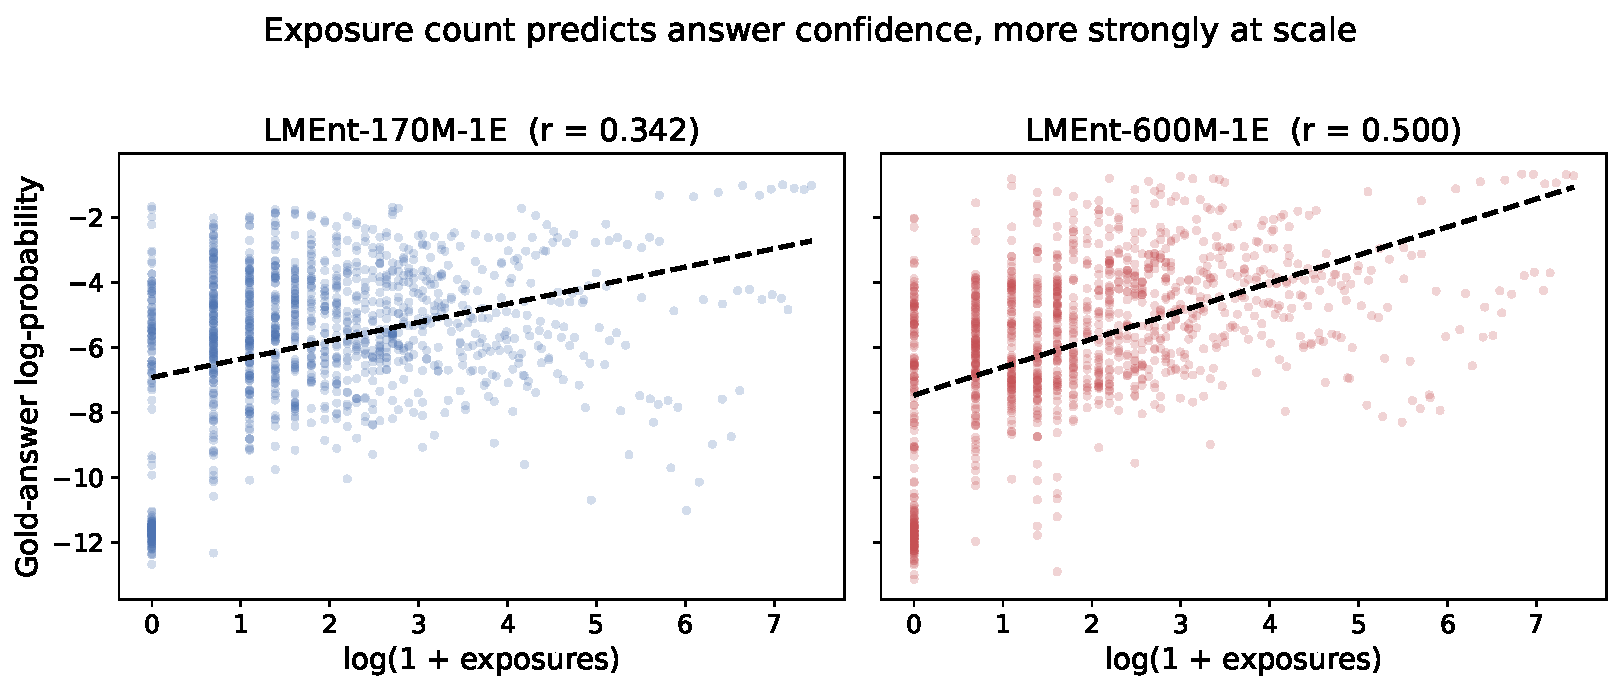
\includegraphics[width=\linewidth]{figures/fig_logprob_vs_exposure.pdf}
  \caption{Gold-answer log-probability vs.\ log(1+exposures), both models. The exposure-confidence relationship is stronger at 600M.}
  \label{fig:logprob}
\end{figure}

\subsection{Accuracy rises, then partially declines, over training}
\label{sec:forgetting}
Both models show a rise-then-partial-decline accuracy trajectory (Figure~\ref{fig:accuracy}): the 170M model peaks around step 20{,}000 (0.49) and falls to 0.42 by the final checkpoint, a drop of about 0.07--0.08; the 600M model peaks around step 50{,}000 (0.44) and ends at 0.41, a smaller and noisier drop of about 0.03. This replicates the forgetting dynamic reported by \citet{chang2024howdo}, using an independent method (per-fact exposure count rather than corpus-level duplication statistics) and a different evaluation (log-probability-based multiple choice rather than exact-match recall). The magnitude of the decline is smaller at 600M than at 170M, suggesting that at least part of this forgetting is a small-model capacity effect that attenuates, rather than persists unchanged, with scale.

\begin{figure}[t]
  \centering
  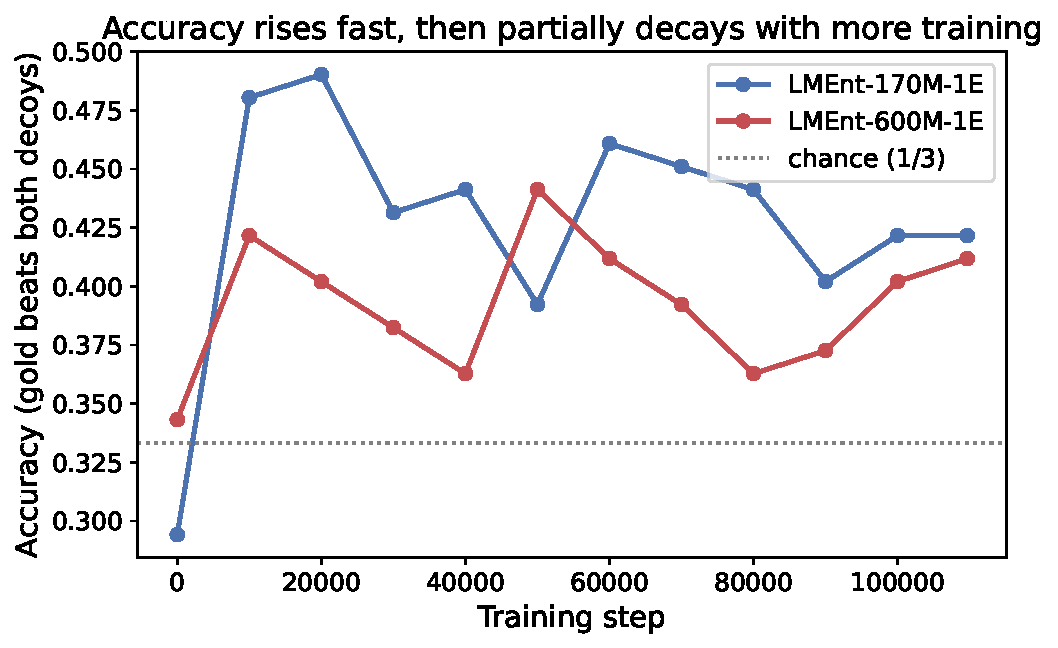
\includegraphics[width=\linewidth]{figures/fig_accuracy_vs_checkpoint.pdf}
  \caption{Accuracy over training steps, both models, against the chance baseline of $1/3$.}
  \label{fig:accuracy}
\end{figure}

\begin{figure}[t]
  \centering
  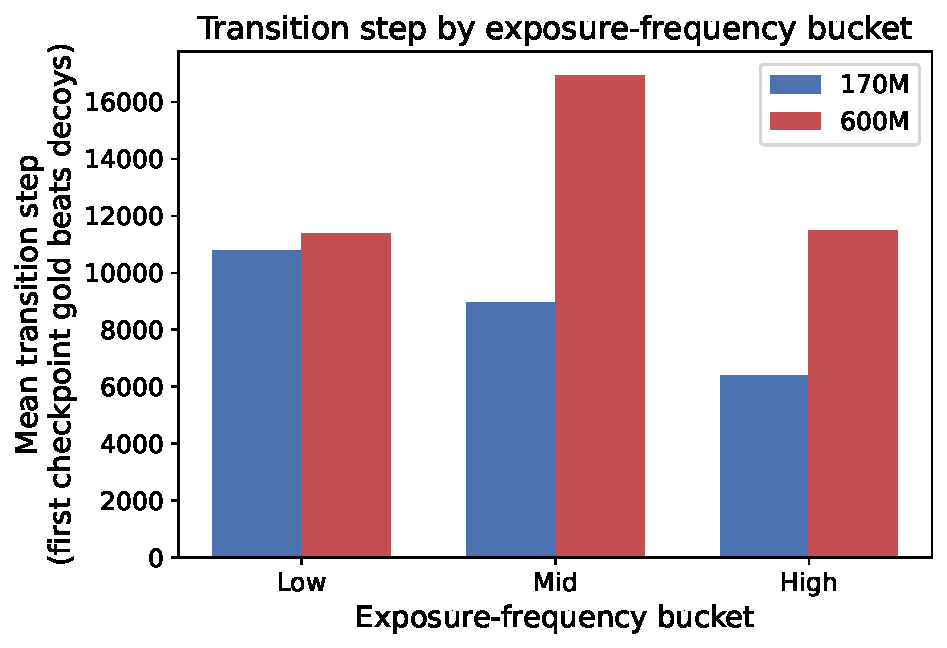
\includegraphics[width=\linewidth]{figures/fig_transition_by_bucket.pdf}
  \caption{Mean transition step by exposure-frequency bucket. The ordering is clean for the 170M model but noisier at 600M.}
  \label{fig:transition}
\end{figure}

\subsection{The forgetting effect is not a decoy artifact}
A natural alternative explanation for the observed decline is that it is an artifact of our evaluation rather than genuine forgetting: perhaps the model develops a generic preference for one particular wrong answer within a relation late in training (e.g.\ always favoring one specific director's name), which would beat many different facts' gold answers regardless of the actual fact being tested. We tested this directly on the 170M results: among facts that were correct at step 20{,}000 but wrong at the final checkpoint (9 facts in this analysis), every single one was beaten by a \emph{different} decoy at the final checkpoint --- no decoy repeats within a relation. This argues against the artifact explanation: the pattern looks like genuine, fact-specific forgetting rather than one systematically over-favored wrong answer contaminating many facts at once.

\subsection{Recency does not explain forgetting: a negative result}
We tested whether a fact's forgetting is explained by \emph{recency} --- whether its supporting chunks were not seen again late in training --- rather than by total exposure count alone. Pooling across all fact--checkpoint pairs with at least one prior exposure, the correlation between recency (training steps since last exposure) and answer confidence is essentially zero ($r=0.011$, $n=1{,}043$). A more targeted comparison, between facts correct at step 20{,}000 but wrong by the final checkpoint (``forgotten,'' $n=12$) and facts correct at both points (``retained,'' $n=38$), is inconclusive: the mean recency gap at the final checkpoint is larger for retained facts (16{,}204 steps) than forgotten facts (11{,}882), but the median goes the other way (6{,}622 vs.\ 8{,}671) --- and both groups are too small to trust either direction. We report this as a genuine negative result: within the granularity available to us (10{,}000-step checkpoints, 102 facts), exposure recency alone does not explain which facts get forgotten. What does remains an open question; Section~\ref{sec:discussion} discusses candidate explanations for future work.

\section{Discussion and Limitations}
\label{sec:discussion}

Our exposure-count result and our forgetting result point in different directions with respect to model scale: the frequency--confidence relationship gets \emph{cleaner} with scale, while the forgetting-over-training effect gets \emph{smaller}. Read together, these suggest that a larger model is both better at cleanly encoding the relationship between how often it saw a fact and how confidently it recalls that fact, and more stable at retaining what it has learned --- two sides of the same underlying capacity story, rather than two unrelated effects.

Several limitations bound how far these claims should be pushed. First, our facts are stratified by \emph{corpus} exposure count, not by an independent notion of real-world popularity, and our decoys are drawn from the same relation but not otherwise matched for difficulty; a harder or easier decoy pool could shift the absolute accuracy numbers, though it should not obviously explain the scale-dependent pattern we observe, since the same sample and decoys were used for both models. Second, our sample (102 facts, 34 per bucket) is large enough to see clean pooled correlations but too small for some finer-grained analyses --- notably the forgotten-vs-retained recency comparison, which had only 12 and 38 facts respectively. Third, we test only one epoch of pretraining and two model sizes (170M, 600M); LMEnt also provides checkpoints for a 1B model and for multiple epochs, which would let us test more directly whether forgetting continues to shrink with further scale, or whether more epochs (more total exposure, but also more opportunity for later data to overwrite earlier associations) changes the picture. Finally, our recency analysis uses checkpoint-level granularity (every 10{,}000 steps); a fact's true ``last seen'' step is known exactly from our exposure timeline, but our correctness labels are only available at the coarser checkpoint resolution, which limits how precisely we can align forgetting to specific exposure events.

\section{Conclusion}
Using LMEnt's exact per-step training provenance, we recover, for individual facts, exactly when and how often a small language model was exposed to them during pretraining, and show that this signal predicts both how quickly a fact is learned and, to a lesser extent, whether it is later forgotten. The frequency--confidence relationship strengthens with model scale (170M to 600M), while the forgetting effect weakens --- a genuine positive result --- and we rule out one plausible artifact explanation for forgetting (a generic decoy bias) while failing to confirm another plausible one (exposure recency), which we report honestly as inconclusive rather than omit.

\section*{AI Disclosure and Reflection}
I used Claude (Claude Sonnet 5, via Claude Code) throughout this project: exploring the LMEnt and \texttt{popqa-kas} data formats and writing the exposure-lookup and evaluation pipeline; debugging real issues that came up while actually running the code (a decoy-methodology flaw that flattened the accuracy curve, a Python string-hashing bug that silently broke a fixed random seed's reproducibility across runs, and a grouping bug that quietly merged two distinct facts sharing a subject name into one during a summary statistic); and setting up and debugging the Slurm/CUDA/PyTorch environment on the university cluster (driver-version and architecture-compatibility mismatches across several attempted package combinations). It was most useful as a hands-on collaborator for exactly this kind of infrastructure debugging, where the fix requires actually running something and reading the real error, not just reasoning about the code. I made the substantive research decisions myself (which exposure signal to use, how to define the decoy comparison, which follow-up analyses to run after each result) and verified every reported number against the underlying result files myself before writing about it here.

\bibliographystyle{acl_natbib}
\bibliography{references}

\end{document}
